\section{Kristalle}
Unter dem Begriff Kristall sollte sich jeder ein Bild machen können. 
Wir werden uns aber nicht auf sein Äusseres fokussieren, sondern was ihn im Inneren ausmacht.
Die Innereien eines Kristalles sind glücklicherweise relativ einfach definiert.
\begin{definition}[Kristall]
    Ein Kristall besteht aus Atomen, welche sich in einem Muster arrangieren, welches sich in drei Dimensionen periodisch wiederholt.
\end{definition}

\begin{figure}
    \centering
    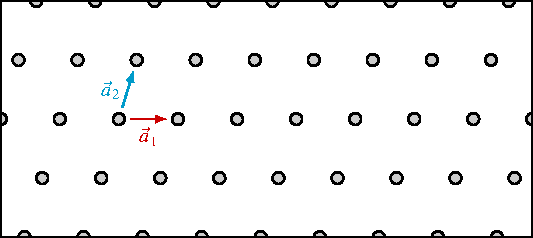
\includegraphics[]{papers/punktgruppen/figures/lattice}
    \caption{
        Zweidimensionales Kristallgitter
        \label{fig:punktgruppen:lattice}
    }
\end{figure}
\subsection{Kristallgitter}
Ein zweidimensionales Beispiel eines solchen Muster ist Abbildung \ref{fig:punktgruppen:lattice}.
Für die Überschaubarkeit haben wir ein simples Motiv eines einzelnen grauen Punktes gewählt und betrachten dies nur in Zwei Dimensionen.
Die eingezeichneten Vektoren $\vec{a}$ und $\vec{b}$ sind die kleinstmöglichen Schritte im Raum bis sich das Kristallgitter wiederholt.
Wird ein beliebiger grauer Gitterpunkt in \ref{fig:punktgruppen:lattice} gewählt und um eine ganzzahlige Linearkombination von $\vec{a}$ und $\vec{b}$ verschoben, endet er zwangsweise auf einem Gitterpunkt, wenn nicht wieder am selben Ort.
Im Dreidimensionalen-Raum können alle Gitterpunkte mit derselben Idee und einem zusätzlichen Vektor $\vec{c}$ also 
\[
    \vec{r} = n_1 \vec{a} + n_2 \vec{b} + n_3 \vec{c}   
\]
erreicht werden sofern $\{n_1,n_2,n_3\} \in \mathbb{Z}$ sind.
Sind die Vektoren  $\vec{a}$ , $\vec{b}$ , $\vec{c}$ gegeben , ist ein Kristallgitter eindeutig beschrieben, weswegen sie  auch als Grundvektoren bekannt sind.

\subsection{Translationssymmetrie}
Da sich das ganze Kristallgitter wiederholt, wiederholen sich auch dessen Eigenschaften periodisch mit den Grundvektoren.
Sollte man sich auf einem Gitterpunkt in einem Kristall aufhalten, ist es unmöglich zu wissen, auf welchem Gitterpunkt man sich befindet, da die Umgebungen aller Punkte Identisch sind. 
Mit anderen worten: Das Kristallgitter $ G $ ist \emph{Translationssymmetrisch} in der Translation 
\[
    Q_i(G) = G + \vec{a_i}
\] wobei der Vektor $a_i$ ein Grundvektor sein muss.
Da die Translationssymmetrie beliebig oft mit allen Grundvektoren angewendet werden kann, können wir auch sagen, dass alle Verschiebungen um eine Linearkombination der Vektoren $\vec{a}$ , $\vec{b}$ und $\vec{c}$ erlaubt sind oder kurz, um $\vec{r}$. 
Verschiebungen um $\vec{r}$ bewirken demnach keine Veränderungen, solange wir ein unendlich grosses Kristallgitter verschieben.

\subsection{Limitierte Kristallsymmetrien}
 Die Translationssymmetrie ist wohl keine grosse Überraschung, wenn man die Abbildung \ref{fig:punktgruppen:lattice} betrachtet.
 Was nicht direkt ersichtlich ist, ist das auch wenn die Grundvektoren frei gewählt werden, können nur Rotationssymmetrische Kristalle erzeugt werden mit Winkel $\alpha \in \{ 0^\circ, 60^\circ, 90^\circ, 120^\circ, 180^\circ\}$.

